% \section{Landmark Discovery}
\paragraph{Part Activations.} In Fig. \ref{fig:shape} we show part activation maps on video sequences from the Penn Action dataset.
\paragraph{Landmark Discovery.} We present unsupervised landmark discovery results on the following datasets: Cat Head (Fig. \ref{fig:kp_cats}), Dogs Run (Fig. \ref{fig:kp_dogs}), CUB-200-2011 (Fig. \ref{fig:kp_birds}), CelebA (Fig. \ref{fig:kp_celeba}), Human3.6M (Fig. \ref{fig:kp_human}) and Penn Action (Fig. \ref{fig:kp_penn}).

\begin{figure}[t]
	\centering
	\includegraphics[trim={0cm 0cm 0cm 0cm},clip, width=1.\linewidth]{fig/supp/shapes}
	\caption{Showing 12 out of 16 part activation maps on Penn Action.}
	\label{fig:shape}
\end{figure}

\begin{figure}[t]
	\centering
	\includegraphics[trim={0cm 0cm 0cm 0cm},clip, width=1.\linewidth]{fig/supp/select48cats}
	\caption{Discovering 10 landmarks on Cat Head.}
	\label{fig:kp_cats}
\end{figure}

\begin{figure}[t]
	\centering
	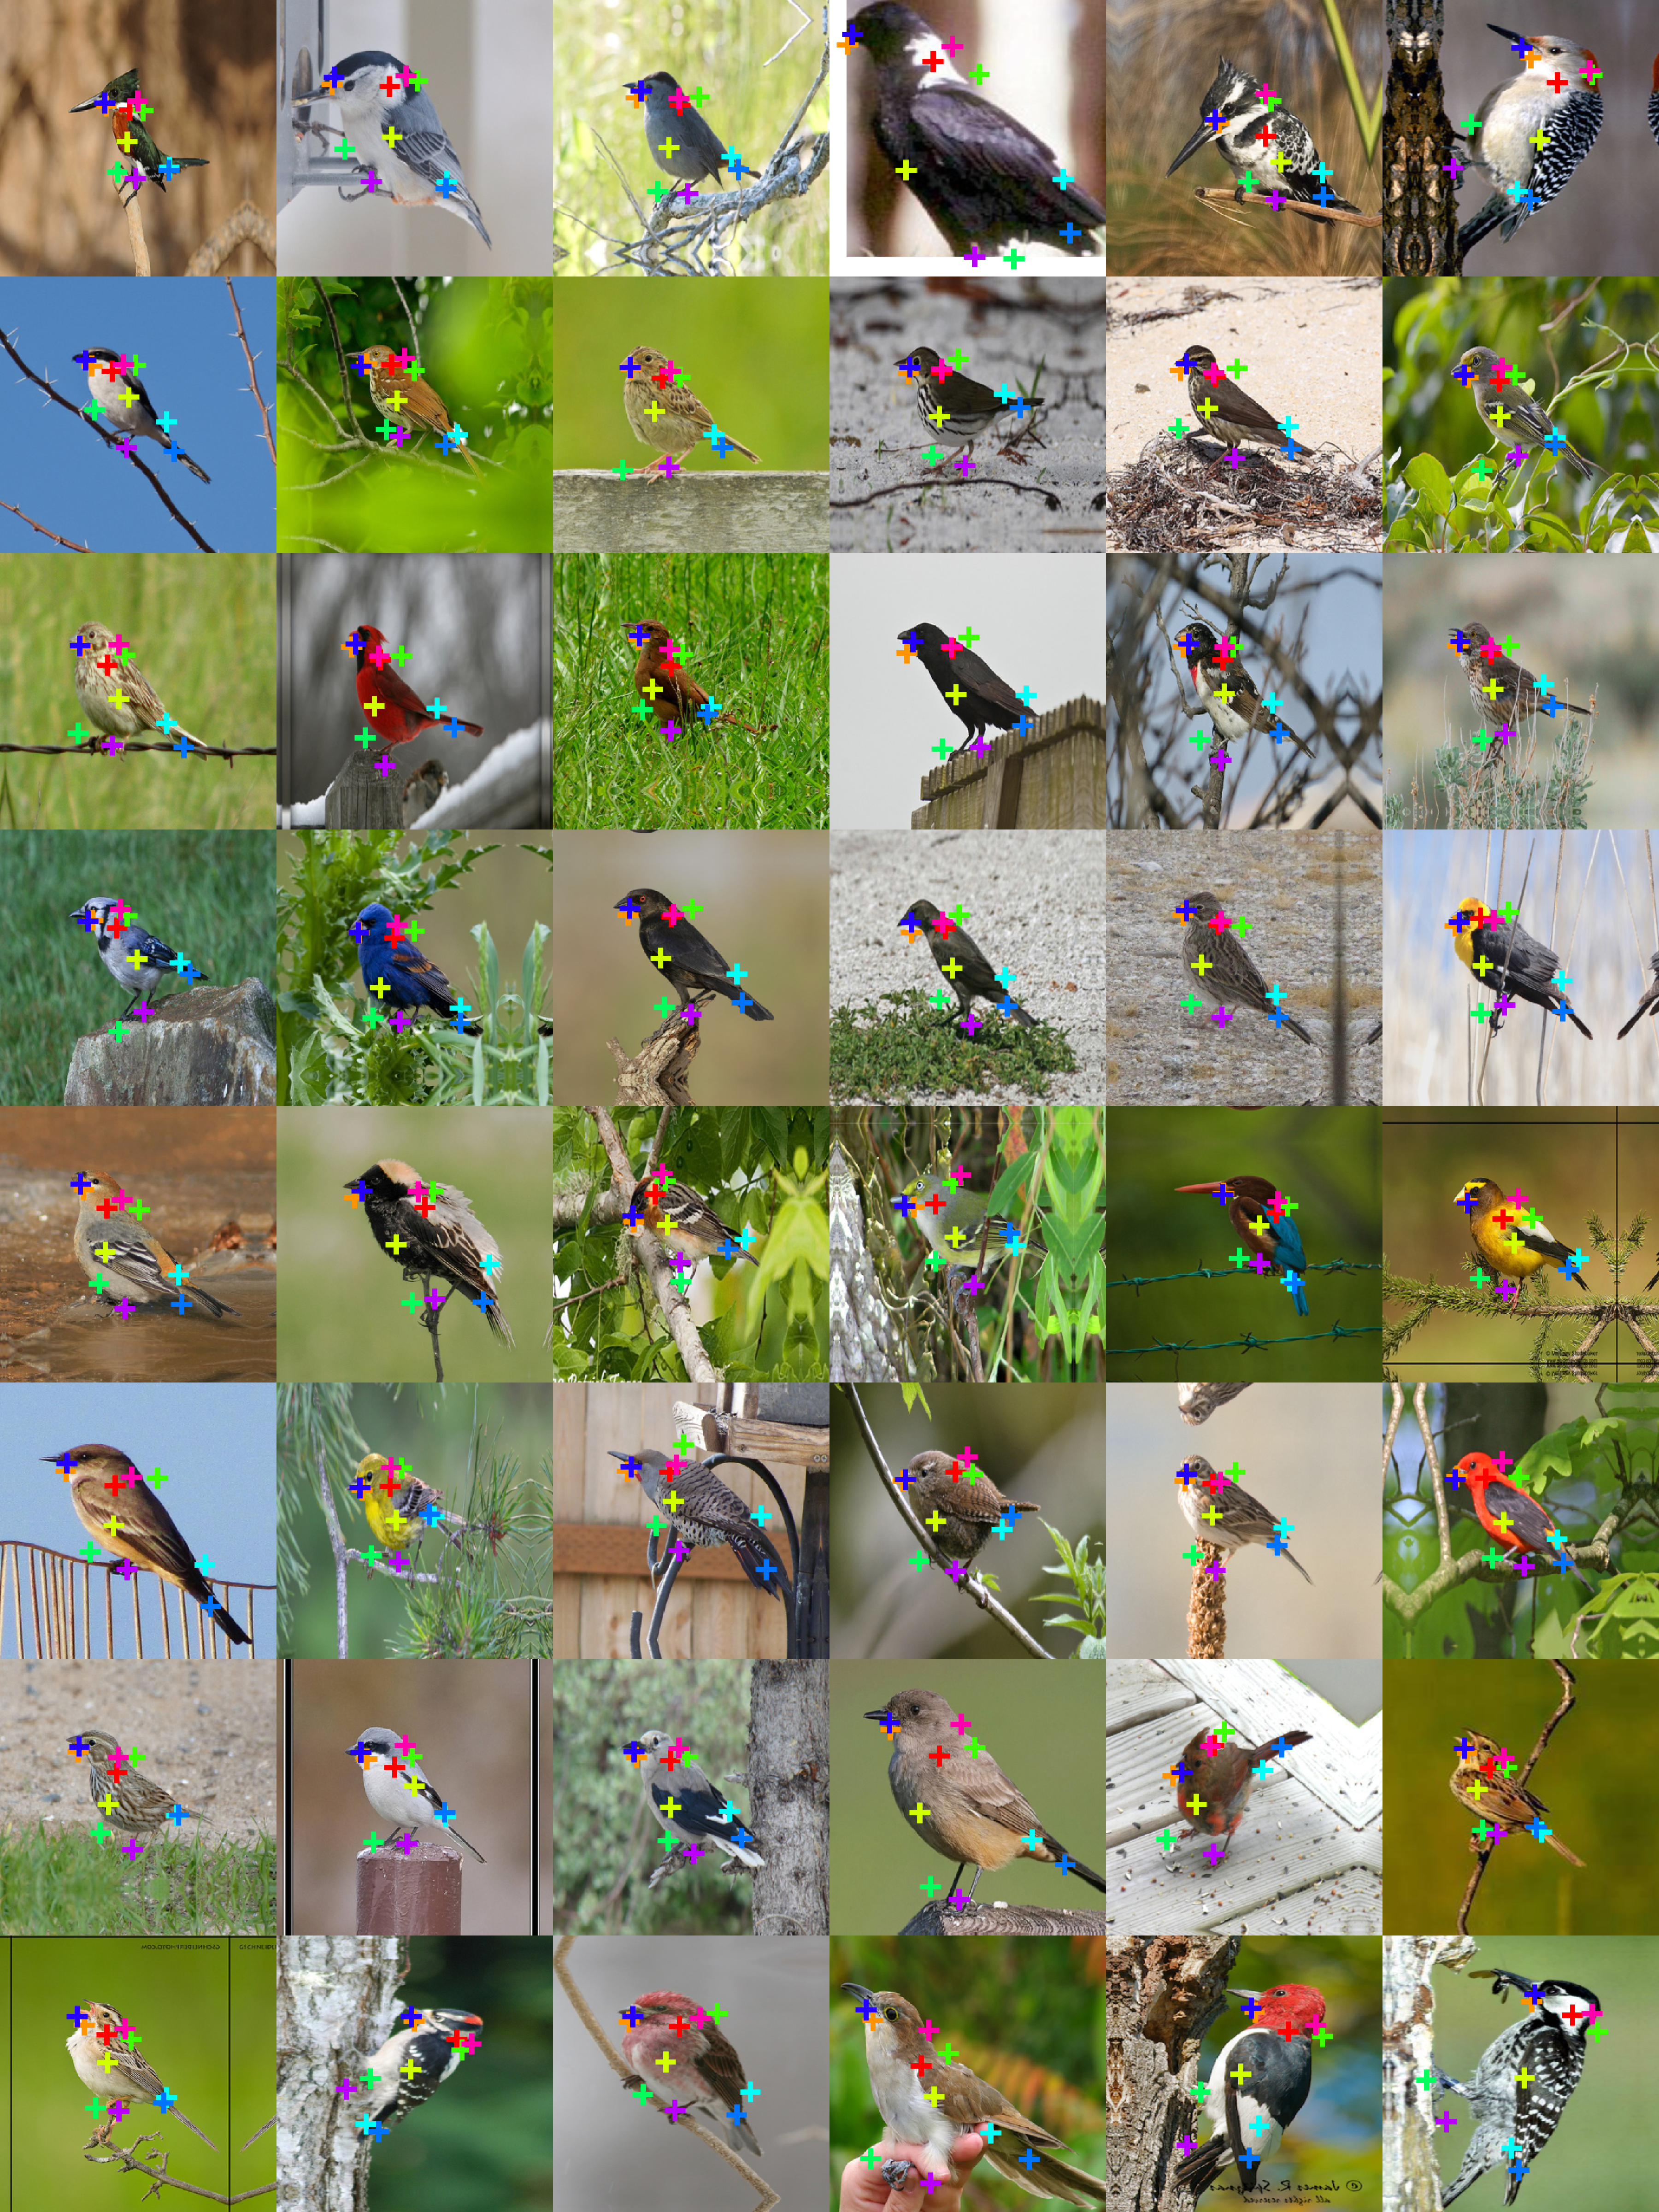
\includegraphics[trim={0cm 0cm 0cm 0cm},clip, width=1.\linewidth]{fig/supp/select48birds}
	\caption{Discovering 10 landmarks on CUB-200-2011..}
	\label{fig:kp_birds}
\end{figure}

\begin{figure}[t]
	\centering
	\includegraphics[trim={0cm 0cm 0cm 0cm},clip, width=1.\linewidth]{fig/supp/select48celeba}
	\caption{Discovering 10 landmarks on CelebA.}\label{fig:kp_celeba}%
	\label{fig:kp_celeba}
\end{figure}

\begin{figure}[t]
	\centering
	\includegraphics[trim={0cm 0cm 0cm 0cm},clip, width=1.\linewidth]{fig/supp/select48human}
	\caption{Discovering 10 landmarks on Human3.6M.}
	\label{fig:kp_human}
\end{figure}

\begin{figure}[t]
	\centering
	\includegraphics[trim={0cm 0cm 0cm 0cm},clip, width=1.\linewidth]{fig/supp/select48penn}
	\caption{Showing 12 out of 16 landmarks on Penn Action.}
	\label{fig:kp_penn}
\end{figure}


